% Get excited! - Senku Ishigami

\documentclass[letterpaper, 8pt]{extarticle}
\usepackage{amssymb,amsmath,amsthm,amsfonts}
\usepackage{multicol,multirow}
\usepackage{calc}
\usepackage{ifthen}
\usepackage[landscape]{geometry}
\usepackage[colorlinks=true,citecolor=blue,linkcolor=blue]{hyperref}

\usepackage{booktabs}
\usepackage{ulem}
\usepackage{enumitem}
\usepackage{tabulary}
\usepackage{graphicx}
\usepackage{siunitx}
\usepackage{tikz}
\usepackage{derivative}
\usepackage{svg}
\usepackage{listings}
\usepackage{setspace}
\usepackage{listings}
\usepackage{xcolor}
\usepackage{courier}
\usepackage{syntax}
\usepackage{mathpartir}
\usepackage{siunitx}
\usepackage{physics}

% minimal line spacing
% \setstretch{0.1}

% set borders (experimentally determined to minimize cutoff and maximize space on school printers)
\geometry{top=.25in,left=.25in,right=.25in,bottom=.35in}

% make figures work better in multicol
\newenvironment{Figure}
{\par\medskip\noindent\minipage}
{\endminipage\par\medskip}

\pagestyle{empty} % clear page

% rewrite section commands to be smaller
\makeatletter
\renewcommand{\section}{\@startsection{section}{1}{0mm}%
                                {-1explus -.5ex minus -.2ex}%
                                {0.5ex plus .2ex}%x
                                {\normalfont\small\bfseries}}
\renewcommand{\subsection}{\@startsection{subsection}{2}{0mm}%
                                {-1explus -.5ex minus -.2ex}%
                                {0.5ex plus .2ex}%
                                {\normalfont\tiny\bfseries}}
\renewcommand{\subsubsection}{\@startsection{subsubsection}{3}{0mm}%
                                {-1ex plus -.5ex minus -.2ex}%
                                {1ex plus .2ex}%
                                {\normalfont\tiny\itshape}}
\makeatother
\setcounter{secnumdepth}{0} % disable section numbering


% disable indenting
\setlength{\parindent}{0pt}
\setlength{\parskip}{0pt plus 0.5ex}

% Custom siunitx defs
\DeclareSIUnit\noop{\relax}
\NewDocumentCommand\prefixvalue{m}{%
\qty[prefix-mode=extract-exponent,print-unity-mantissa=false]{1}{#1\noop}
}

% Shorthand definitions
\newcommand{\To}{\Rightarrow}
\newcommand{\ttt}{\texttt}
\newcommand{\ra}{\rightarrow}

% condense itemize & enumerate
\let\olditemize=\itemize \let\endolditemize=\enditemize \renewenvironment{itemize}{\olditemize \itemsep0em}{\endolditemize}
\let\oldenumerate=\enumerate \let\endoldenumerate=\endenumerate \renewenvironment{enumerate}{\oldenumerate \itemsep0em}{\endoldenumerate}
\setlist[itemize]{noitemsep, topsep=0pt, leftmargin=*}
\setlist[enumerate]{noitemsep, topsep=0pt, leftmargin=*}

% make matricies narrower
\setlength{\arraycolsep}{0pt}

\title{3SP3}

\begin{document}
\raggedright
\tiny

% make listings look nicer
\lstset{
    tabsize = 2, %% set tab space width
    showstringspaces = false, %% prevent space marking in strings, string is defined as the text that is generally printed directly to the console
    basicstyle = \tiny\ttfamily, %% set listing font and size
    breaklines = true, %% enable line breaking
    numberstyle = \tiny,
    postbreak = \mbox{\textcolor{red}{\(\hookrightarrow\)}\space}
}

\begin{center}
    {\textbf{3SP3 Final - Rocinante Edition}} \\
\end{center}
% set column spacing rules
\setlength{\premulticols}{1pt}
\setlength{\postmulticols}{1pt}
\setlength{\multicolsep}{1pt}
\setlength{\columnsep}{2pt}
\begin{multicols*}{5}
\begin{tabular}{| c | c | c |}
    \hline
    \textbf{Factor} & \textbf{Prefix} & \textbf{Symbol} \\
    \hline
    $10^{12}$ & tera & T \\
    $10^{9}$ & giga & G \\
    $10^{6}$ & mega & M \\
    $10^{3}$ & kilo & k \\
    $10^{-3}$ & milli & m \\
    $10^{-6}$ & micro & $\mu$ \\
    $10^{-9}$ & nano & n \\
    $10^{-12}$ & pico & p \\
    \hline
\end{tabular}
\section{Intro}
\textbf{System}:
Combination of interacting elements organized
to achieve a stated purpose or meet an operational need.
\textbf{System Boundary}:
Defines separation of system of interest and operating environment.
\textbf{Interface}:
Input / Output that flows across system boundaries.
\textbf{Mission}:
A problem that a system intends to solve.
Should be clearly defined by the stakeholder acquiring the system.

\textbf{Life Cycle}
\textbf{Conceptualization}:
Defining requirements.
E.g. what does the market want?
What type of product are we building?
What features do we want?
\textbf{Realization}:
Taking requirements, making design.
Building factories, tooling, prototypes, enter full production.
\textbf{Utilization}:
Processes during the use of the system.
Marketing / sales, maintenance, warranty, recalls, feedback.
\textbf{Retirement}:
End-of-life services.
Recycling, special disposal, updating / disposing of tooling.

\subsection{Systems Engineering Overview}
Top-down approach to design, development, operation of systems.
Iterative, repeats for each lower level until individual elements are defined.
Used because good planning and clear definition of deliverables makes sure that
stakeholder needs and engineering solutions are aligned.

\subsection{Project Life Cycle}
\textbf{Pre-Phase A}:
Concept Studies.
Generate ideas for new missions, draft system concepts.
Establish needs, goals, objectives. Assess feasibility.
\textbf{Phase A}:
Concept and Technology Development.
Develop mission into requirements, system architecture.
Identify technology development required.
\textbf{Phase B}:
Preliminary Design.
Develop system concept into design solution meeting mission needs.
Finish technology development.
\textbf{Phase C}:
Final Design and Fabrication.
Complete detailed design, procure or fabricate components.
Establish procedures, controls for manufacture.
\textbf{Phase D}:
Assembly, Integration, Test, Launch.
Assemble subsystems, integrate,
test to verify and validate system against requirements, deploy.
\textbf{Phase E}:
Operations and Sustainment.
Put system into service.
\textbf{Phase F}:
Closeout.
End of life operations, analysis. Retire system.

\textbf{Stakeholders}:
Groups that are affected or have an interest/stake in program or project.
\textbf{Need}:
A single statement clearly describing what the customer wants.
Domain of customer. Independent of specific solution / implementation.
System is not the need, but response to need.
E.g. ``The Government of Canada needs a more effective means of monitoring shipping traffic in the arctic.''
\textbf{Goals}:
Elaboration of need, setting specific expectations on system.
Qualitative expressions of what system will accomplish.
E.g. ``Provide rapid detection of vessel traffic in Canadian arctic waters.''
\textbf{Objectives}:
Specific target outputs system must achieve.
Specific, Measurable, Attainable, Relevant, Time-Bound.
Quantitative extension of goals.
E.g. ``Detect any surface vessel entering Canadian arctic territorial waters within 1 hour.''
\textbf{Measures of Effectiveness}:
Metrics to judge whether a mission is successful in meeting objectives / achieving goals.
Stated from stakeholder's POV.
E.g. ``No undetected vessels appearing inside 50 nm of Canadian arctic territorial waters.''
(Not directly observable by design team, each MOE assigned 1+ \textit{Measures of Performance},
defining level of perf system must meet to enable MOE.)
\textbf{Constraints}:
Boundaries placed on system design. Usually one of
technical, performance, resources, environmental,
schedule, cost, regulatory, organizational.
\textbf{Concept of Operations}:
Document that outlines high-level vision \& strategy for use \& operation of a system to achieve intended goals.
Who are the stakeholders?
What is the mission?
What is the proposed solution?
How will it be used?
Where will it be used?
By whom?
Over what time?
\textit{Context Diagram}:
Shows mission, system scope.
\textit{Timeline}:
Shows time sequence of operations.
Can identify weak spots, e.g. unacceptable gaps in coverage.
\textbf{Mission Requirements}:
Formal statements defining capabilities, functions, performance, operating condition for system to meet goals, objectives.
Requirements can be validated (demonstrated to be true).
Mission requirements starting point for system requirements.

\section{Requirements}
\subsection{Requirements Engineering}
Process of translating stakeholder expectations into technical statements
usable by design team to make a solution that meets the original need.
Bridges gap between stakeholder expectations, design teams technical instructions.

\subsection{Why requirements}
Tell us what our system needs to do.
Tell us scope of system.
Give opportunity for every stakeholders' input to be captured.
Help structure, scope work to be done, estimating effort and cost.
Allow us to track project progress.
How we know we are done, how well we did.

Separate from the "Needs View", directly define the input to design.

\textbf{Requirement = input to design. Specification = output of design.}

\subsection{Internal Requirements}
Self-imposed, usually during R\&D, early product development.
Will evolve, change during early project life-cycle.

\subsection{External Requirements}
Defined by the customer, contractor must abide by these.
Changes are more difficult and require more evidence, approvals.
Various formats, stated order of precedence.
E.g. contract, statement of work, technical requirements,
product assurance requirements.

\subsection{Requirement}
Formally written, agreed upon statement of what the system must do,
a quality it must posess,
or a constraint it must operate under in order to meet the need.
``The <system name> shall <system response>''

\textbf{Shall:} a statement of requirement. This must be met.
\textbf{Should:} a statement of a goal or non-mandatory request. Desired, but not required.
\textbf{Will:} a statement of fact, declaration of purpose.

\subsubsection{Functional Requirements:}
What functions need to be performed to accomplish objective.
System as a ``black box'' of functions.
Focus on \textit{what} needs to be done, not \textit{how} to do it.

\subsubsection{Non-functional Requirements:}
Other properties the system must posess, constraints it must operate under.
Performance, environment, interfaces, constraints, ``-ilities'', training, personnel, safety.

\textbf{Performance:}
How well the system should perform functions.
How much / little, how far, how fast, how many, how often\dots
E.g. bit error rates.

\textbf{Environmental Requirements:}
Requirements defining operating system of system. E.g. shock exposure levels, operating temperatures.

\textbf{Interface Requirements:}
How elements interface with other elements internal / external to system.
(Accepting inputs, providing outputs are functional, but specifics on how the interface should work are not)
E.g. what standard of communication is used between systems.

\textbf{Constraints}
Limitations, boundaries, conditions imposed on system by stakeholders.
Include cost, timeline, physical dimension, quantity (size, weight, power), rules and regulations.

\textbf{-ilities}
Deal with life-cycle considerations product quality, other stakeholders.
Relability, availability, scalability, maintainability, operabiliy, supportability, security, manufacturability, interoperability, etc.
Major design, cost drivers.

\subsection{Good Requirements}
Good requirements should be
\begin{itemize}
    \item Needed (should be necessary, sufficient to specify system. Nothing extraneous.)
    \item Verifiable (must have a clear pass/fail criteria, a method to determine if it is met)
    \item Attainable (no point in requiring the impossible)
    \item Traceable (must be linked from the lowest component to the highest need)
\end{itemize}
Good requirements are also good comms:
Single thought, concise, simple ad consistent, grammatically correct.

\subsection{Requirement Documentation}
Requirement ID, Title, Requirement Text, Rationale, Verification, Tracability, Notes.

\subsubsection{Requirement Rationale}
Additional information on intent, context for a requirement, helps with interpretation.
Reason for the requirement.
Documents assumptions made when writing requirement.
Link to supporting information outside requirement set, e.g. architecture decisions, ConOps, trade studies, customer discussions, etc\dots

\subsubsection{Requirement Verification}
Reqs need to be verified.
\begin{itemize}
    \item Inspection: visual examination of product, supporting documentation
    \item Demonstration: using product to demonstrate requirement is met
    \item Analysis: use of modelling, simulation, analytical techniques to predict a product will meet requirement
    \item Test: highly controlled use, measurement of product to compare to pass/fail criteria
\end{itemize}

\subsubsection{Requirement Traceability}
Ability to trace every requirement to it's source.
Most come from other requirements, not always.
ALso applies to ConOps, architecture documents, trade studies, analysis, other documentation.

\textbf{Forwards Traceability:} Relationship of parent requirements down to children.
\textbf{Backwards Traceability:} Relationship of child requirements up to their parents.

\subsection{Requirement Validation}
Ensure the requirements capture stakeholder's expectation.
Ensure are complete and correct,
accurately capturing the stakeholder needs,
necessary,
achievable,
not duplicated or over-specified,
verifiable.

\subsection{Why manage requirements}
Requirements will evolve as system evolves.
Complex projects have hundreds of requirements, allocated across many elements, multiple developers.

\section{Systems Engineering}
% TODO: CUT ME IF U NEED SPACE
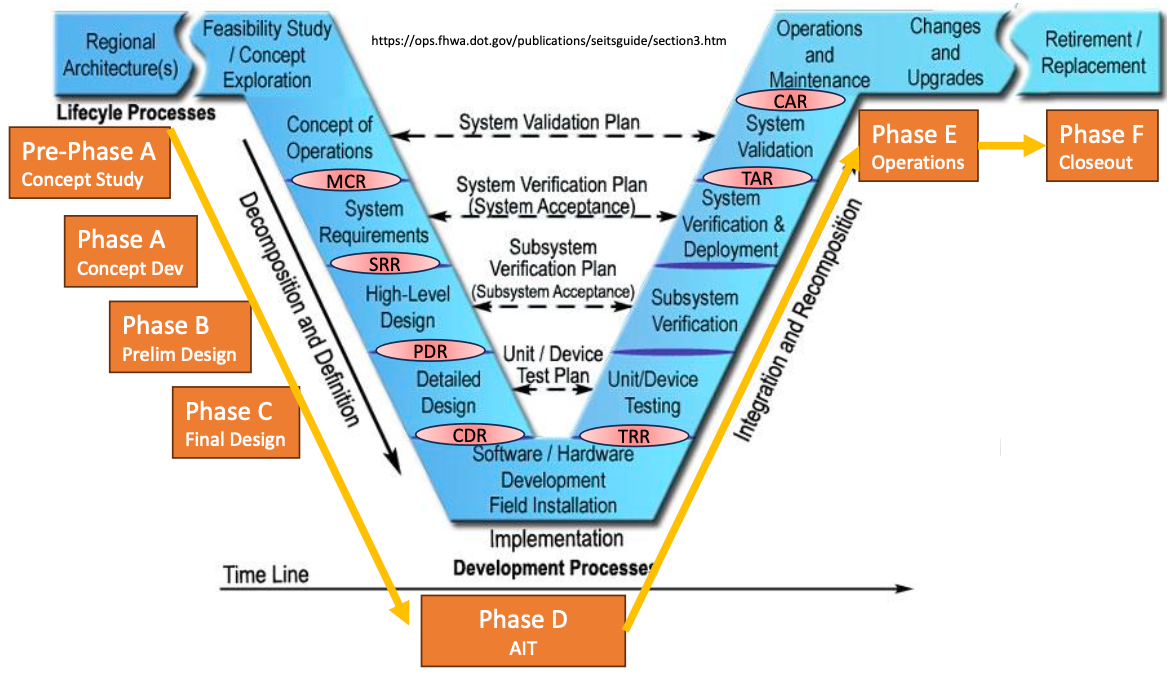
\includegraphics[width=\linewidth]{SCR-20241218-ouqp.png}
System Design Process:
Analysis, Synthesis, Evaluation.

\textbf{ConOps:} Operations Concept (aka a diagram)

\textbf{NASA System Design Process}
\textbf{1. Stakeholder Expectation Definition:}
Identify stakeholders, expectations, requirements. Capture expectations in ConOps. Identify Measures of Effectiveness.
\textbf{2. Technical Requirements Definition:}
Turn stakeholder expectations into formal technical statements used to further decompose, define system.
Identify system scope (what are we responsible for, what are we not responsible for), system boundary (physical manifestation of scope).
Identify interfaces. Define functions to use system, as identified in ConOps.
\textbf{Elicitation:} Drawing out, e.g. stakeholder telling us, recieving it from a source.
\textbf{Elaboration:} Further develop existing requirements using Decomposition (breaking it down into smaller parts) or Derivation (making inferences and creating new requirements).
\textbf{3. Logical Decomposition:}
Problem has been defined, now prepare to solve it.
Decompose problem into smaller parts (logical or functional).
Proposing architecture as candidate solution to decomposed problem.
Allocating functional decomposition to elements in architecture.
Deriving further requirements.
Evaluating proposed solution.
Iterating to find best overall solution for need.
Finalizing all requirements to bring to design.
\textbf{4. Design Solution Definition:}
Translate requirements into design. (Most course work / lab work, here is a problem solv it.)
Propose and analyze multiple potential solutions.
Selected alternative fully defined into complete design solution.

\section{Launch Environment}
\textbf{Thrust Equation:}
$T = \dot{m_e} v_e + (p_e - p_a)A_e$
\textbf{Rocketry Equation:}
$\Delta v = I_{sp} g_0 \ln \frac{m_0}{m_f}$
\textbf{Design for Launch}
Max Q: peak dynamic pressure.
Rocket vibration from thrust, static load/random vibration, structural resonance.
Acoustic vibration from atmospheric forces.
Resonance and dampening:
Q is ratio of output displacement to input.
Generally aluminum is used.
Thermal baance, we want $Q_{in} = Q_{out}$,
where $Q_{out} = Q_{solar} + Q_{albedo} + Q_{EarthIR} + Q_{spacecraft}$.
(Albedo is reflection of sun from Earth.)

Test thermal properties using TVAC (thermal vaccum chamber), heat lamps to simulate solar / albedo loading.

\section{Quality}
\textbf{Quality:} How to make sure that your solution meets safety/reliability standards?
Guard against failure.
Plan -> Do -> Check -> Act -> Repeat.
Performed by Product Assurance -> Quality Assurance -> Quality Control -> Audit.
QC: Inspecting work to ensure quality is maintained.
QA: Process control, ensuring process is in place, maintain documentation and traceability for audits.
Manufacturing, test data to verify something conforms to engineering data.
Process to identify, prevent defects.
Plans, implements systematic activities to provide confidence that all quality requirements will be fulfilled.
PA: Make sure product meets specifications, including quality, assurance. ``Voice of customer''.
Ensure project is built per process using ``stuff'' that meets customer requireents.
Proposal -> design -> manu -> test -> deliv -> commissioning.
Certificat of Conformance (indicates deliverable built and tested per reqs.)

PA Requirement e.g.: EEE Components (Electrical, Electronic, or Electromechanical)
must either be on an approved list or be approved,
must be purchased from approved manufacturers,
components must also pass specifications,
must pass qualification.

E.g. NASA EEE-INST-002:
Level 1: Lowest risk, highest reliability.
Level 2: Low to moderate risk.
Level 3: Higher risk.
Commercial.
Higher level = higher standards, testing, can be an order of magnitude more expensive.
Lower quality components need to undergo additional testing to be accepted.

\textbf{5. Product Realization}
Design is done, SE switches to ``bottom-up'',
building smallest components first up to largest.
Usually either build, buy, or reuse, based on skills, capability, experience, cost, etc.
Can buy by paying a contractor to build (more requirements need to be exchanged),
or purchase COTS (existing stuff that is higher risk).
COTS is hard to qualify, lower performance. Can test new parts on case-by-case basis.
Reusing is usually attractive, especially if it has worked in space before.
\textbf{Assembly:} joining individual components together to make higher level products.
\textbf{Integration:} combining elements to achieve a higher level function. Must include some level of ``using'' product to enable the purpose.
Integration ensures different subsystems work together properly.
\textbf{Test:} Test as you go, make sure each part works.

\textbf{6. Product Integration}
Assemble, Integrate, Test until full system is done.
Systems plans for AIT in design, sees it through here.
Quality makes sure build quality is maintainted, tests are performed properly.

\textbf{7. Product Verification}
Did we build it right?

Model philosiphies
Breadboard: test model, cheap components, partial designs.
Engineering model: CLose to flight, cheaper parts, less functionality.
Engineering Qualification Model: Close to flight, cheaper parts, full functionality.
Qualification Model: Identical to flight, flight component, flight process.
Proto-Flight Model: Full functionality, qualified parts, materials, process.
Tested to higher requirements to check margin.
Only on first flight deliverable.
Flight model: Same as proto-flight model, tested to normal requirements.

\textbf{8. Product Validation}
Did we build the right system?
Does it meet the needs of the customers / users?

\textbf{Validation vs Verification}
Verification: Did we build the system how we said we would?
Validation: Stakeholder expectations (MOEs, and MOPs)

\textbf{9. Product Transition}

\textbf{10-17. Technical Management}

\section{Satellite Systems}
\noindent\textbf{Primary Uses of Space:} Communication, navigation, observation, exploration, and experimentation. Examples include communication systems like Intelsat 40e and SpaceX Starlink; navigation systems like GPS; observation systems such as Radarsat 2 and Sentinel; and exploration missions like Artemis/Orion, ISS, and the James Webb Space Telescope (JWST).
\noindent\textbf{A Systems View of Satellites:} Satellites extend the system boundary to space, requiring enabling products such as launch vehicles and ground stations. They host payloads to perform system functions in orbit.
\noindent\textbf{System Design Drivers:} Key drivers include:
Cost, which impacts parts, testing equipment, and personnel;
Schedule, limiting design, testing, and component availability;
Orbit, affecting thermal, radiation, and atmospheric conditions;
Lifetime, driving redundancy and reliability requirements;
Payload, supporting interfaces, power, orientation, and data flow;
Volume and Mass, dictated by the launcher;
and Power, determined by orbit and influencing solar panels, batteries, and power distribution.
\noindent\textbf{Satellite Functional Hierarchy:} Satellites are divided into two primary elements:
The \textbf{Payload}, which provides the mission capability (e.g., GPS clocks, imaging sensors); and
The \textbf{Bus}, which supports the payload with power, thermal control, orbit and attitude control, and communication.
\noindent\textbf{Key Subsystems:} These include:
\textbf{Structure}, which supports satellite components and interfaces with the launcher;
\textbf{Thermal Control}, which maintains system temperatures using radiators and heat pipes;
\textbf{Power}, which provides energy via solar panels, batteries, and distribution systems;
\textbf{Propulsion}, which adjusts orbit and orientation using chemical, cold gas, or electric systems;
\textbf{Attitude Control}, which ensures stability and pointing with sensors and actuators (e.g., reaction wheels, star trackers);
\textbf{Data Handling}, which manages commands, telemetry, and mission data; and
\textbf{Communications}, which links the satellite to ground stations for telemetry and payload data.

\section{Space Environment}
\textbf{1. Near-Earth Radiation Environment:}
\textbf{Van Allen Belts:} Inner Belt (high-energy protons/electrons, $\sim$1,000-6,000 km). Outer Belt (high-energy electrons, $\sim$9,000 km to beyond geostationary orbit).
\textbf{South Atlantic Anomaly (SAA):} Region of lower magnetic field where radiation penetrates to lower altitudes; can disrupt electronics.
\textbf{Solar Influence:} Solar cycles ($\sim$11 years): Maximum increases flares and CMEs; minimum increases trapped particles.
\textbf{2. Cosmic Rays:}
High-energy particles from outside the solar system, partially deflected by Earth's magnetic field.
\pagebreak
\textbf{3. Radiation Effects:}
\textbf{On Materials:} Degrades optics, structural components, and electrical parts.
\textbf{Types of Effects:} TID (long-term degradation), SEE (immediate damage, e.g., bit flips, hardware failures).
\textbf{4. Mitigation Strategies:}
\textbf{Radiation Shielding:} Straight-line and Monte Carlo models (e.g., Geant).
\textbf{Designing for Tolerance:} Use radiation-hardened components and fail-safe designs.
\textbf{5. Thermal Considerations:}
\textbf{LEO:} Rapid cycling between sunlight ($\sim+120^\circ$C) and shadow ($\sim-100^\circ$C) every 90 minutes.
\textbf{GEO:} Longer thermal transition periods due to 24-hour orbits.
\textbf{6. Plasma and Charging:}
Plasma from solar storms or Earth's magnetosphere can cause charging and electrostatic discharge, damaging systems.

\section{Math}
\textbf{Dot Product}:
$\vec{a} \cdot \vec{b} = a_x b_x + a_y b_y + a_z b_z = |\vec{a}| |\vec{b}| \cos \theta$;
$|\vec{a}|^2 = \vec{a} \cdot \vec{a}$.
\textbf{Projection}:
$proj_{\vec{b}} \vec{a} = \frac{\vec{a} \cdot \vec{b}}{|\vec{b}|} \frac{\vec{b}}{|\vec{b}|} = \frac{\vec{a} \cdot \vec{b}}{\vec{b} \cdot \vec{b}}\hat{b}$;
$\vec{a}_{\perp \vec{b}} = \vec{a} - proj_{\vec{b}}\vec{a}$.
\textbf{Cross Product}:
$\vec{a} \times \vec{b} = (a_y b_z - a_z b_y)\hat{i} - (a_x b_z - a_z b_x)\hat{j} + (a_x b_y - a_y b_x)\hat{k}$;
$\hat{n}_{ab} = \frac{\vec{a} \times \vec{b}}{|\vec{a} \times \vec{b}|}$;
$\vec{a} \times \vec{b} = |a| |b| \sin \theta \hat{n}_{ab}$.
\textbf{Matrix x Vector Multiplication}:
\includegraphics[width=0.7\linewidth]{matrix\_vec\_mult\_as\_process.png}

\section{Orbital Mechanics}
% TODO: see if i'm missing anything here
\subsection{2D}
\textbf{Kepler's Laws}
K1 - Orbit of planet is ellipse, Sun at one of two foci.
K2 - Line segment joining planet, Sun sweeps out equal areas during equal intervals of time.
K3 - Square of planet's orbital period proportional to cube of length of semi-major axis of orbit.

\subsubsection{Forces}
$\vec{F} = m \vec{a} = \odv{\vec{p}}{t}$.
$\vec{p} = m \vec{v}$.
\textbf{Impulse on mass $m$:} (change in momentum when acted upon by a force)
$I = \int_{t_1}^{t_2} \vec{F} \dd{t} = m \vec{v}_2 - m \vec{v}_1$.
$\Delta \vec{v} = I / m = F_{net} \Delta t / m$ (if $F_{net}$ const).
\textbf{Gravitational Constant:}
$G = 6.67430 \times 10^{-11} \, \frac{\text{Nm}^2}{\text{kg}^2}$.

\subsubsection{Rotation, Torque, Angular Momentum}
\textbf{Torque (moment) on mass m:} $\vec{M_0} = \vec{r} \times \vec{F} = \odv{\vec{H_0}}{t}$
\textbf{Angular Momentum:} $\vec{H_0} = \vec{r} \times m \vec{v} = \vec{r} \times \vec{p}$

\subsubsection{Orbits}

\textbf{Two-body equation of motion:}
$\mu = G(m_1 + m_2)$ (gravitational param);
$\ddot{\vec{r}} = -\frac{G(m_1 + m_2)}{r^3} \vec{r} = - \frac{\mu}{r^3}\vec{r}$.

\textbf{Angular Momentum:} $\vec{h} = \vec{r} \times \vec{v}$ \si{\kilo\gram\metre\per\second} (convert to \si{\kilo\gram\kilo\metre\per\second} if needed)

\textbf{Eccentricity vector}: $\vec{e} = \frac{\vec{C}}{\mu}$
\textbf{Orbit Equation}:
$\boxed{r = \frac{h^2}{mu} \frac{1}{1 + e \cos \theta}}$

\subsubsection{Circular Orbit $e = 0$}
$r = h^2 / \mu = \mu / v^2$;
$h = r v_\perp$;
$v = v_\perp$;
$v_{circ} = \sqrt{\frac{\mu}{r}}$;
$T_{circ} = \frac{2 \pi}{\sqrt{mu} r^{3/2}}$

\subsubsection{Orbital Constants}
$G = 6.67430 \times 10^{-20}$ \si{\newton\kilo\metre\squared\per\kilo\gram\squared};
$R_E = 6378$ \si{\kilo\metre};
$M_E = 5.97219 \times 10^{24}$ \si{\kilo\gram};
$\mu = G(M_e + M_s) \approx G(M_e) \approx 398600$ \si{\kilo\metre\cubed\per\second\squared};

\subsubsection{Elliptical Orbit $0 < e < 1$}
$r = \frac{h^2}{\mu} \frac{1}{1 + e \cos \theta} = \frac{a (1 - e^2)}{1 + e \cos \theta}$. \\
\textbf{Periapsis}: Closest approach. \\
\textbf{Apoapsis}: Furthest approach. $a + c$ away from the mass at focal point. \\
\textbf{Semimajor axis}: $a = \frac{h^2}{\mu} \frac{1}{1 - e^2}$ (the longer one) \\
\textbf{Semiminor axis}: $b = a \sqrt{1 - e^2}$ (the shorter one) \\
\textbf{Linear eccentricity}: $c = a e$ \\
\textbf{Semilatus rectum}: $p = \frac{h^2}{\mu}$ \\
\textbf{True anomaly}: $\theta$, the degree of rotation from periapsis. \\
\textbf{Specific Energy of $m2$ (constant)}: $\epsilon = -\frac{1}{2} \frac{\mu}{h^2}(1 - e^2)$. \\
\textbf{Orbit Period}: $T_{ellipse} = \frac{2 \pi a b}{h} = \frac{2 \pi a^{3/2}}{\sqrt{\mu}}$, \\
where $b = a \sqrt{1 - e^2}, h = \sqrt{\mu a(1-e^2)}$ \\

\subsubsection{Parabolic Trajectory $e = 1$, Hyperbolic Trajectory $e > 1$}
$v_{esc} = \sqrt{2} v_{circ}$, arrive at inifinity with 0 velocity.
$v_\infty^2 = v^2 - v_{esc}^2$, arrive at inifinity with velocity $v_\infty$.

\subsubsection{Perifocal Frame}
Coordinate frame where orbit lies in XY plane.
\begin{itemize}
    \item Centered at the focus
    \item X axis points along apse line to periapsis (0 true anomaly)
    \item Y axis along semilatus rectum
    \item Z axis in normal direction of angular momentum $\vec{\mathbf{h}}$
\end{itemize}

$r = \frac{h^2}{\mu} \frac{1}{1 + e \cos(\theta)},
x = r \cos \theta, y = r \sin \theta
$

$\vec{\mathbf{r}} = x \, \hat{\mathbf{p}} + y \, \hat{\mathbf{q}}$

$\vec{\mathbf{r}} = \frac{h^2}{\mu} \frac{1}{1 + e \cos(\theta)} 
\left( \cos(\theta) \, \hat{\mathbf{p}} + \sin(\theta) \, \hat{\mathbf{q}} \right)$

$\vec{\mathbf{v}} = \dot{x} \, \hat{\mathbf{p}} + \dot{y} \, \hat{\mathbf{q}}$

$\vec{\mathbf{v}} = \frac{\mu}{h} 
\left( -\sin(\theta) \, \hat{\mathbf{p}} + (e + \cos(\theta)) \, \hat{\mathbf{q}} \right)$

\subsubsection{Orbit Relationships}
$2a = r_a + r_p$;
$e = \frac{r_a - r_p}{r_a + r_p}, \frac{r_p}{r_a} = \frac{1-e}{1+e}$;
$a = \frac{h^2}{\mu} \frac{1}{1 - e^2}$;
$h = \sqrt{\mu a (1 - e^2)} = r_a v_{\perp a} = r_p v_{\perp p}$;

$r_a = \frac{h^2}{\mu} \frac{1}{1-e}$;
$r_p = \frac{h^2}{\mu} \frac{1}{1+e}$;

$v_\perp = \frac{\mu}{h}(1 + e \cos \theta)$
$v_r = \frac{\mu}{h} e \sin \theta$


\subsubsection{Orbit Energy}

\subsubsection{Lagrange Coefficients}
$h = |\vec{r_0} \times \vec{v_0}|$;
$v_{r0} = \vec{v_0} \cdot \frac{\vec{r_0}}{r_0}$;
$r = \frac{h^2}{\mu} \frac{1}{1 + \left(\frac{h^2}{\mu r_0} - 1\right) \cos(\Delta \theta) - h \frac{v_{r0}}{\mu} \sin(\Delta \theta)}$

$f = 1 - \frac{\mu r}{h^2} (1 - \cos(\Delta \theta)), g = \frac{r r_0}{h} \sin(\Delta \theta)$ \\
$\dot{f} = \frac{\mu}{h} \frac{1 - \cos(\Delta \theta)}{\sin(\Delta \theta)} \left[\frac{\mu}{h^2} (1 - \cos(\Delta \theta)) - \frac{1}{r_0} - \frac{1}{r}\right]$
$\dot{g} = 1 - \frac{\mu r_0}{h^2} (1 - \cos(\Delta \theta))$

\textbf{Therefore,}
$\vec{r} = f \vec{r_0} + g \vec{v_0}$;
$\vec{v} = \dot{f} \vec{r_0} + \dot{g} \vec{v_0}$

Solving for eccentricity, initial true anomaly:
$r_0 = \frac{h^2}{\mu} \frac{1}{1 + e \cos(\theta_0)}$
$v_{r0} = \frac{\mu}{h} e \sin(\theta_0)$

\subsubsection{Orbit Position as a Function of Time}
Circle:
$\theta(t) = \frac{\mu^2}{h^3} t, t(\theta) = \frac{h^3}{\mu^2} \theta$

Elliptical Orbit:
$M_e = t \frac{\mu^2}{h^3} (1 - e^2)^{3/2}$\\
$E = 2 \tan^{-1} \left(\sqrt{\frac{1 - e}{1 + 3}} \tan(\frac{\theta}{2})\right)$\\
$e \sin E = \frac{e \sqrt{1 - e^2} \sin(\theta)}{1 + e \cos(\theta)}$\\
$M_e = E - e \sin E = \frac{2 \pi t}{T_{orbit}}$\\
(given $\theta$ solve for $t$ directly, or $\theta \to E \to M_e \to t$)

\subsection{3D}
\textbf{Sidereal Rate:} Rotation rate of Earth relative to ``fixed stars'',
$\omega_E = 7.292115 \times 10^{-5}$ \si{rad\per\second}.
\textbf{Right Ascention:} Degrees east along equator from vernal equinox.
\textbf{Declination:} Latitude north from equator.

\subsubsection{Geocentric Equatorial Frame}
Coordinate frame is fixed, used to rep satellite position, velocity.
\textbf{X axis} along direction of vernal equinox (at chosen epoch!)
\textbf{Z axis} along Earth's axis of rotation (at chosen epoch!)
\textbf{Y axis} completes cartesian coordinate system.
Precession, Nutation of the Earth spin axis causes it to drift over time, so epoch matters.
(Precession: Earth's axis rotating around a central axis, Nutation: variations / wiggles in precession)

\subsubsection{Orbital Parameters}
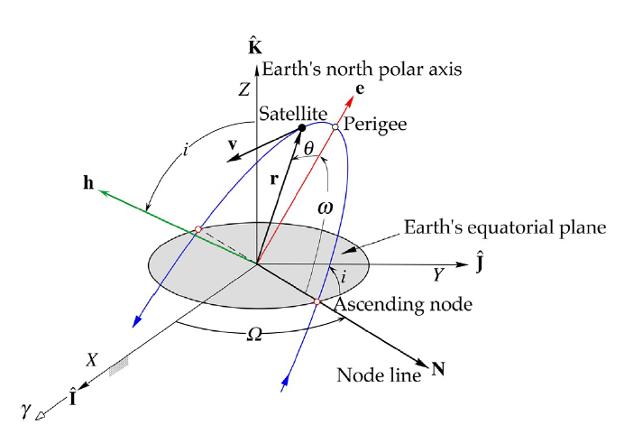
\includegraphics[width=.7\linewidth]{3D Orbital Parameters.png}
Given Position and Velocity vectors, we can calculate orbital elements:

\begin{enumerate}
    \item Distance: $r = \sqrt{\vec{r} \cdot \vec{r}}$
    \item Speed: $v = \sqrt{\vec{v} \cdot \vec{v}}$
    \item Radial velocity: $v_r = \frac{\vec{r}}{r} \cdot \vec{v}$
          ($v_r > 0$ away from perigee, $v_r < 0$ towards perigee)
    \item Specific angular momentum: $\vec{h} = \vec{r} \times \vec{v}$
          (magnitude $h = \sqrt{\vec{h} \cdot \vec{h}}$)
    \item Inclination: $i = \cos^{-1} (h_Z / h)$
        ($0^\circ \leq i < 90^\circ$: prograde orbit (same direction as Earth rotation),
        $90^\circ < i \leq 180^\circ$: retrograde orbit (opposite direction to Earth rotation))
    \item Node line: $\vec{N} = \hat{K} \times \vec{h}$
        (Magnitude $N = \sqrt{\vec{N} \cdot \vec{N}}$)
    \item RAAN: $\Omega = \cos^{-1} (N_X / N)$
        ($N_Y \geq 0, \Omega = \cos^{-1} (N_X / N)$,
        $N_Y < 0, \Omega = 360^\circ - \cos^{-1}(N_X / N)$)
    \item Eccentricity vector: $\vec{e} 
        = \frac{\vec{v} \times \vec{h}}{\mu} - \frac{\vec{r}}{r}
        = \frac{1}{\mu} \left[\left(v^2 - \frac{\mu}{r}\right) \vec{r} - r v_r \vec{v}\right]$
        (Magnitude: $e = \sqrt{\vec{e} \cdot \vec{e}}$)
    \item Argument of perigee: $\omega = 
    \begin{cases}
        e_Z \geq 0 & \cos^{-1} \left(\frac{\vec{N}}{N} \cdot \frac{\vec{e}}{e}\right) \\
        e_Z < 0 & 360^\circ - \cos^{-1} \left(\frac{\vec{N}}{N} \cdot \frac{\vec{e}}{e}\right) \\
    \end{cases}$
    \item True Anomaly: $\theta =
    \begin{cases}
        v_r \geq 0 & \cos^{-1} \left(\frac{\vec{e}}{e} \cdot \frac{\vec{r}}{r}\right) \\
                   & \text{or } \cos^{-1} \left(\frac{1}{e} \left[\frac{h^2}{\mu r} - 1\right]\right) \\
        v_r < 0    & 360^\circ - \cos^{-1} \left(\frac{\vec{e}}{e} \cdot \frac{\vec{r}}{r}\right) \\
                   & \text{or } 360^\circ - \cos^{-1} \left(\frac{1}{e} \left[\frac{h^2}{\mu r} - 1\right]\right) \\
    \end{cases}$
\end{enumerate}

\subsubsection{Perifocal to ECI Frame}

$
\vec{\mathbf{r}} = \frac{h^2}{\mu} \frac{1}{1 + e \cos(\theta)} 
\begin{bmatrix}
\cos(\theta) \\
\sin(\theta) \\
0
\end{bmatrix}
$

$
\vec{\mathbf{v}} = \frac{\mu}{h}
\begin{bmatrix}
- \sin(\theta) \\
e + \cos(\theta) \\
0
\end{bmatrix}
$

\subsubsection{2D Rotations}

\subsubsection{3D Rotations}

\textbf{Euler Z-X-Z:}
$
(\alpha, \beta, \gamma) \to R_Z(\gamma) R_X{\beta} R_Z(\alpha)
\mid \alpha \in [0^\circ, 360^\circ], \beta \in [0, 180^\circ], \gamma \in [0^\circ, 360^\circ]
$

\scalebox{0.8}{$\vec{v}_{x' y' z'} =$}
\scalebox{0.8}{$
\begin{bmatrix}
    \cos \gamma & \sin \gamma & 0 \\
    -\sin \gamma & \cos \gamma & 0 \\
    0 & 0 & 1
\end{bmatrix}
\begin{bmatrix}
    1 & 0 & 0 \\
    0 & \cos \beta & \sin \beta \\
    0 & -\sin \beta & \cos \beta \\
\end{bmatrix}
\begin{bmatrix}
    \cos \alpha & \sin \alpha & 0 \\
    -\sin \alpha & \cos \alpha & 0 \\
    0 & 0 & 1 \\
\end{bmatrix}
\vec{v}_{xyz}
$}

\scalebox{0.7}{$Q_{ZXZ} =$}
% scalebox abuse to get this to fit
\scalebox{0.7}{$
\begin{bmatrix}
-\sin\alpha \cos\beta \sin\gamma + \cos\alpha \cos\gamma & \cos\alpha \cos\beta \sin\gamma + \sin\alpha \cos\gamma & \sin\beta \sin\gamma \\
-\cos\alpha \cos\beta \sin\gamma - \cos\alpha \sin\gamma & \cos\alpha \cos\beta \cos\gamma - \sin\alpha \sin\gamma & \sin\beta \cos\gamma \\
\sin\alpha \sin\beta & -\cos\alpha \sin\beta & \cos\beta
\end{bmatrix}
$}

\textbf{Yaw-Pitch-Roll:}
$
(\alpha, \beta, \gamma) \to R_X(\gamma) R_Y(\beta) R_Z(\alpha)
\mid \alpha \in [0, 360^\circ], \beta \in (-90^\circ, 90^\circ), \gamma \in [0^\circ, 360^\circ]
$

\scalebox{0.7}{$\vec{v}_{x' y' z'} =$}
\scalebox{0.7}{$
\begin{bmatrix}
    1 & 0 & 0 \\
    0 & \cos \gamma & \sin \gamma \\
    0 & -\sin \gamma & \cos \gamma \\
\end{bmatrix}
\begin{bmatrix}
    \cos \beta & 0 & -\sin \beta \\
    0 & 1 & 0 \\
    \sin \beta & 0 \cos \beta \\
\end{bmatrix}
\begin{bmatrix}
    \cos \alpha & \sin \alpha & 0 \\
    -\sin \alpha & \cos \alpha & 0 \\
    0 & 0 & 1
\end{bmatrix}
\vec{v}_{xyz}
$}

\scalebox{0.7}{$Q_{YPR} =$}
\scalebox{0.7}{$
\begin{bmatrix}
\cos\alpha \cos\beta & \sin\alpha \cos\beta & -\sin\beta \\
\cos\alpha \sin\beta \sin\gamma - \sin\alpha \cos\gamma & \sin\alpha \sin\beta \sin\gamma + \cos\alpha \cos\gamma & \cos\beta \sin\gamma \\
\cos\alpha \sin\beta \cos\gamma + \sin\alpha \sin\gamma & \sin\alpha \sin\beta \cos\gamma - \cos\alpha \sin\gamma & \cos\beta \cos\gamma
\end{bmatrix}
$}

\textbf{Perifocal to Geocentric Equatorial}
$
Q_{GCE \to pfc} = R_Z(\omega) R_X(i) R_Z(\Omega)
$

\begin{normalsize}
    \scalebox{0.54}{$
    Q_{pfc \to GCE} = Q_{XYZ \to pqw}^T = R_Z(-\Omega) R_X(-i) R_Z(-\omega) =
    $}
    \scalebox{0.54}{$
    \begin{bmatrix}
        -\sin\omega \cos i \sin\Omega + \cos\omega \cos\Omega & -\cos\omega \cos i \sin\Omega - \sin\omega \cos\Omega & \sin i \sin\Omega \\
        \cos\omega \cos i \sin\Omega + \cos\omega \sin\Omega & \cos\omega \cos i \cos\Omega - \sin\omega \sin\Omega & -\sin i \cos\Omega \\
        \sin\omega \sin i & \cos\omega \sin i & \cos i
    \end{bmatrix}
    $}
\end{normalsize}

\subsubsection{Oblateness}
\textbf{Regression of Node:}
$
\dot{\Omega} = -\left[
    \frac{3}{2} \frac{\sqrt{\mu} J_2 R^2}{(1 - e^2)^2 a^{7/2}}
\right] \cos i
$

\textbf{Advance of Perigee:}
$
\dot{\omega} = -\left[
    \frac{3}{2} \frac{\sqrt{\mu} J_2 R^2}{(1 - e^2)^2 a^{7/2}}
\right]
\left(
    \frac{5}{2} \sin^2 i - 2
\right)
$

\subsection{Date-related 3D}
Latitude and Longitude to Cartesian Coordinates

(Radius of line from point at perpendicular height $H$ above reference surface to polar axis)
$R_\phi = \frac{R_E}{\sqrt{1 - (2f - f^2) \sin^2 \phi}}$

$R_{xyz} = 
\begin{bmatrix}
    (R_\phi + H) \cos \phi \cos \Lambda \\
    (R_\phi + H) \cos \phi \sin \Lambda \\
    ((1 - f^2) R_\phi + H) \sin \phi
\end{bmatrix}
$
$H$: Altitude of coordinate\\
$f = (R_E - R_P) / R_E$: Flattening factor of oblate spheroid\\
$R_E$: Equatorial radius of the Earth\\
$R_P$: Polar radius\\
$\phi$: Geodic Latitude\\
$\Lambda$: Geodic Longitude\\

\textbf{WGS84 Reference Ellipsoid}\\
$R_E =$ \SI{6378137.0}{\metre}\\
$f = 1/298.257\,223\,563$ \\
$R_P \approx$ \SI{6356752.314245}{\metre}\\

\textbf{Julian Date Formula}\\
$JD = JD_0 + \frac{UT}{24}$\\
$JD_0 = 367y
- \left\lfloor\frac{7(y - \left\lfloor\frac{m + 9}{12}\right\rfloor)}{4}\right\rfloor
+ \left\lfloor\frac{275m}{9}\right\rfloor
+ d
+ 1\,721\,013.5$\\

\textbf{Sidereal Time}\\
\textbf{Centuries since J2000:}
$T_0 = \frac{JD_0 - 2\,451\,545}{36\,525}$\\
\textbf{Greenwich sidereal time at 0 UT:}
$\theta_{G_0} = 100.460\,618\,4
+ 36\,000.770\,04 T_0
+ 0.000\,387\,933 T_0^2
- 2.583 \times 10^{-8} T_0^3
(deg)$\\
\textbf{Greenwich sidreal time at current time in UT:}
$\theta_G = \theta_{G_0} + 360.985\,647\,24 \frac{UT}{24}$\\
\textbf{Local sidereal time:}
$\theta_{SD} = \theta_G + \Lambda$.

To go from Earth-Centered-Earth_fixed to Earth-Centered-Inertial,
we need to perform a Z axis frame rotation from ECEF to ECI by sidereal time.
AKA, we need to rotate by $-\theta_G$.

\section{Satellite Communications}
Channel Capacity:
$
C = BW \log_2 \left(1 + \frac{S}{N}\right)
$ \si{\bit\per\second}
BW: bandwidth, S: signal, N: noise.
SNR: $\frac{S}{N} = \frac{P_{sig}}{P_{noise}} = \frac{P_{sig}}{N_0 BW}$
($N_0$ is power spectral density of noise (e.g. \si{\watt\per\hertz}).
Usually associated with thermal noise in system,


\textbf{Symbol Rate:} $R_S = \frac{1}{T_S} = BW$ (inverse of time the symbol takes up)

\textbf{Average Energy per Symbol:} $E_S = \frac{1}{M} \sum_{i=1}^M \int_{-\infty}^{\infty}|s_i (t)|^2 dt$

\textbf{Average Power:} $P_s = E_S R_S$

\textbf{Probability of Error:} $p_e = Q\left(\frac{s_1 - s_0}{\sigma_1 + \sigma_0}\right) = Q\left(\frac{d}{2 \sigma}\right)$
$p_{e, OOK} = Q\left(\sqrt{\frac{E_b}{N_0}}\right) = Q(\sqrt{SNR_{lin}})$
$p_{e, BPSK} = Q\left(\sqrt{\frac{2 E_b}{N_0}}\right) = Q(\sqrt{2 SNR_{lin}})$

\subsection{Link Budget Equation}
\textbf{Base SI units:} $P_{RX} = P_{TX} L_{TX} G_{TX} L_{FS} L_P G_{RX} L_{RX}$

\textbf{Logarithmic units:} $P_{RX} (dBm) = P_{TX} (dBm) - L_{TX} (dB) + G_{TX} (dB) - L_{FS} (dB) - L_P (dB) + G_{RX} (dB) - L_{RX} (dB)$

\textbf{Linear to Logarithmic:} $X_dB = 10 \log_{10} X_{lin}$, and $P_{dBm} = 10 \log_{10} \frac{P_{lin}}{1 mW}$
(\SI{1}{\milli\watt} = \SI{0.001}{\watt})

\subsubsection{Antenna Gain}
RF antennas:
$l(r) = \frac{P}{4 \pi r^2} \frac{W}{m^2}$
Gain for all power concentrated in area S: $G = \frac{4 \pi r^2}{S}$
E.g.
Parabolic antenna (high directivity): $G_{par} = \frac{4 \pi A}{\lambda^2} e_A = \left(\frac{\pi d}{\lambda}\right)^2 e_A$
aperture diameter $d$, wavelength $\lambda$, aperture efficiency factor $e_A$.

Optical antenna directional gain scales with wavelength:
$G_{Tx} = \left(\frac{\pi D}{\lambda}\right)^2$

\subsubsection{Antenna Coverage} (not used in calc?)
$\theta = \frac{kd}{\lambda}$,
$G_{par} = \left(\frac{\pi k}{\theta}\right)^2 e_A$

\subsubsection{Free Space Loss}
$L_{free} = \left(\frac{\lambda}{4 \pi d}\right)^2$,
$L_{free_{DB}} = 20 \log_{10} \left(\frac{\lambda}{4 \pi d}\right)$.

\subsubsection{Pointing Loss}
\textbf{RF Antennas} \\
1/2 power BW: $\theta_{3dB} \approx \frac{70^\circ \lambda}{D}$,
and pointing loss: $L_{point}(dB) \approx -12 \left(\frac{\Delta \theta}{\theta_{3dB}}\right)^2$

\textbf{Optical Antennas} \\
$1/e^2$ intensity profile BW:
$\theta_{div} \approx \frac{\lambda}{\pi \omega_0}$,
and pointing loss: $L_{point}(dB) \approx -8.7 \left(\frac{\Delta \theta}{\theta_{div}}\right)^2$

\textbf{Reciever Gain}
Same as above for transmitter, just update variables for reciever antenna.

\subsubsection{Reciever Noise}
$P_{th, RF} = k_b TBW$, or in dBm, $P_{th} (dbm) = -174 \frac{dB}{Hz} + 10 \log_10 BW$

\subsubsection{Noise Figure}
$N_f$, How much extra noise is injected by reciever electronics.

\subsubsection{Desired SNR}
$SNR_{BER} = P_{Rx} - P_{noise} = P_{Rx} + 174 - 10 \log_{10} BW - N_f$

Because optical interferometers are hard,
$SNR_{opt} = \bar{n_s} = \frac{P_{Rx}}{hvR_s}$
$h =$ \SI{6.62607015e-34}{\joule\per\hertz}

\section{Satellite Attitude \& Orbit Control Systems}
\textbf{ADCS Subsystem:}
System to estimate spacecraft body orientation,
determine error,
process spacecraft dynamics to formulate corrective commands,
command actuators to perform adjustements.

\subsection{Attitude Sensing}
Estimate of current spacecraft orientation from sensor measurements

\subsection{Sun Sensor}
Orients at the sun.
$\alpha = \tan^{-1} \frac{\Delta X}{h}$,
$\beta = \tan^{-1} \frac{\Delta Y}{h}$.

\subsection{Horizon Sensor}
Uses local horizon to orient towards Earth
Earth is warm versus space.
Horizon depends on altitude, so use a wider FOV for lower orbits.

\subsection{Star tracker}
$star_{pos} (x_i, y_i) = (f \tan \theta, f \tan \phi)$.

\section{Spacecraft Dynamics}
How to go from orbital parameters to state vectors?

\begin{enumerate}
    \item Given orbital parameters, calculate $r, v$ in perifocal frame:
    $
    \{\mathbf{r}\}_{\bar{x}} = \frac{h^2}{\mu} \frac{1}{1 + e \cos \theta}
    \begin{Bmatrix}
    \cos \theta \\
    \sin \theta \\
    0
    \end{Bmatrix}
    \quad
    \{\mathbf{v}\}_{\bar{x}} = \frac{\mu}{h}
    \begin{Bmatrix}
    -\sin \theta \\
    e + \cos \theta \\
    0
    \end{Bmatrix}
    $
    \item Calculate matrix Q (e.g. Euler zxz)
    $
    [\mathbf{Q}]_{\bar{x}\bar{X}} = 
    \begin{bmatrix}
    \cos \omega & \sin \omega & 0 \\
    -\sin \omega & \cos \omega & 0 \\
    0 & 0 & 1
    \end{bmatrix}
    \begin{bmatrix}
    1 & 0 & 0 \\
    0 & \cos i & \sin i \\
    0 & -\sin i & \cos i
    \end{bmatrix}
    \begin{bmatrix}
    \cos \Omega & \sin \Omega & 0 \\
    -\sin \Omega & \cos \Omega & 0 \\
    0 & 0 & 1
    \end{bmatrix}
    $
    \item Re-calculate $r, v$ in ECI frame
    $
    \{\mathbf{r}\}_{X} = [\mathbf{Q}]_{\bar{x}X} \{\mathbf{r}\}_{\bar{x}}
    \quad
    \{\mathbf{v}\}_{X} = [\mathbf{Q}]_{\bar{x}X} \{\mathbf{v}\}_{\bar{x}}
    $
\end{enumerate}

\subsection{Rigid Body Dynamics}

\textbf{Rotating Body time derivatives of vector (orbit)}
Given that $\vec{\omega} = \odv{\theta}{t}$ and $\vec{\alpha} = \odv{\vec\omega}{t}$

$
\odv{\vec{A}}{t} = \vec{\omega} \times \vec{A}
$
and
$
\odv[2]{\vec{A}}{t} = \vec{\alpha} \times \vec{A} + \vec{\omega} \times (\vec{\omega} \times \vec{A})
$

\textbf{Time derivative of moving vector in body frame}
Given that $\vec{B} = [B_x \hat{I} + B_y \hat{J} + B_z \hat{K}] (inertial) = [b_x \hat{j} + b_y \hat{j} + b_z \hat{k}] (rotating frame)$

We have
$
\odv{\vec{B}}{t} = \odv{b_x}{t} \hat{i} + \odv{b_y}{t} \hat{j} + \odv{b_z}{t} \hat{k} + \vec{\omega} \times \vec{B}
$
i.e. the time derivative of $\vec{B}$ in inertial frame is equal to the time derivative of $\vec{B}$ in the rotating frame,
plus the correction term $\vec{\omega} \times \vec{B}$.

% TODO:
% Translation
% Moment
% Angular Momentum
% Angular Momentum Impulse
% Rigid Body Angular Momentum
% Moment of inertia
% Moment of inertia matrix


\end{multicols*}

\end{document}
